%%
%% This is file `sample-manuscript.tex',
%% generated with the docstrip utility.
%%
%% The original source files were:
%%
%% samples.dtx  (with options: `manuscript')
%%
%% IMPORTANT NOTICE:
%%
%% For the copyright see the source file.
%%
%% Any modified versions of this file must be renamed
%% with new filenames distinct from sample-manuscript.tex.
%%
%% For distribution of the original source see the terms
%% for copying and modification in the file samples.dtx.
%%
%% This generated file may be distributed as long as the
%% original source files, as listed above, are part of the
%% same distribution. (The sources need not necessarily be
%% in the same archive or directory.)
%%
%% Commands for TeXCount
%TC:macro \cite [option:text,text]
%TC:macro \citep [option:text,text]
%TC:macro \citet [option:text,text]
%TC:envir table 0 1
%TC:envir table* 0 1
%TC:envir tabular [ignore] word
%TC:envir displaymath 0 word
%TC:envir math 0 word
%TC:envir comment 0 0
%%
%%
%% The first command in your LaTeX source must be the \documentclass command.
%%%% Small single column format, used for CIE, CSUR, DTRAP, JACM, JDIQ, JEA, JERIC, JETC, PACMCGIT, TAAS, TACCESS, TACO, TALG, TALLIP (formerly TALIP), TCPS, TDSCI, TEAC, TECS, TELO, THRI, TIIS, TIOT, TISSEC, TIST, TKDD, TMIS, TOCE, TOCHI, TOCL, TOCS, TOCT, TODAES, TODS, TOIS, TOIT, TOMACS, TOMM (formerly TOMCCAP), TOMPECS, TOMS, TOPC, TOPLAS, TOPS, TOS, TOSEM, TOSN, TQC, TRETS, TSAS, TSC, TSLP, TWEB.
% \documentclass[acmsmall]{acmart}

%%%% Large single column format, used for IMWUT, JOCCH, PACMPL, POMACS, TAP, PACMHCI
% \documentclass[acmlarge,screen]{acmart}

%%%% Large double column format, used for TOG
% \documentclass[acmtog, authorversion]{acmart}

%%%% Generic manuscript mode, required for submission
%%%% and peer review
\documentclass[review, sigplan]{acmart}
\usepackage{listings}
\usepackage{cleveref}
%% Fonts used in the template cannot be substituted; margin
%% adjustments are not allowed.
%%
%% \BibTeX command to typeset BibTeX logo in the docs
%\AtBeginDocument{%
%  \providecommand\BibTeX{{%
%    \normalfont B\kern-0.5em{\scshape i\kern-0.25em b}\kern-0.8em\TeX}}}

%% Rights management information.  This information is sent to you
%% when you complete the rights form.  These commands have SAMPLE
%% values in them; it is your responsibility as an author to replace
%% the commands and values with those provided to you when you
%% complete the rights form.
%\setcopyright{acmcopyright}
%\copyrightyear{2018}
%\acmYear{2018}
%\acmDOI{XXXXXXX.XXXXXXX}

%% These commands are for a PROCEEDINGS abstract or paper.
%\acmConference[Conference acronym 'XX]{Make sure to enter the correct
%  conference title from your rights confirmation emai}{June 03--05,
%  2018}{Woodstock, NY}
%
%  Uncomment \acmBooktitle if th title of the proceedings is different
%  from ``Proceedings of ...''!
%
%\acmBooktitle{Woodstock '18: ACM Symposium on Neural Gaze Detection,
% June 03--05, 2018, Woodstock, NY}
%\acmPrice{15.00}
%\acmISBN{978-1-4503-XXXX-X/18/06}


%%
%% Submission ID.
%% Use this when submitting an article to a sponsored event. You'll
%% receive a unique submission ID from the organizers
%% of the event, and this ID should be used as the parameter to this command.
%%\acmSubmissionID{123-A56-BU3}

%%
%% For managing citations, it is recommended to use bibliography
%% files in BibTeX format.
%%
%% You can then either use BibTeX with the ACM-Reference-Format style,
%% or BibLaTeX with the acmnumeric or acmauthoryear sytles, that include
%% support for advanced citation of software artefact from the
%% biblatex-software package, also separately available on CTAN.
%%
%% Look at the sample-*-biblatex.tex files for templates showcasing
%% the biblatex styles.
%%

%%
%% The majority of ACM publications use numbered citations and
%% references.  The command \citestyle{authoryear} switches to the
%% "author year" style.
%%
%% If you are preparing content for an event
%% sponsored by ACM SIGGRAPH, you must use the "author year" style of
%% citations and references.
%% Uncommenting
%% the next command will enable that style.
%%\citestyle{acmauthoryear}

%%
%% end of the preamble, start of the body of the document source.
\begin{document}

%%
%% The "title" command has an optional parameter,
%% allowing the author to define a "short title" to be used in page headers.
\title{Cobb: Synthesis of Test Input Generators with Coverage Types}

%%
%% The "author" command and its associated commands are used to define
%% the authors and their affiliations.
%% Of note is the shared affiliation of the first two authors, and the
%% "authornote" and "authornotemark" commands
%% used to denote shared contribution to the research.
\author{Patrick LaFontaine}
\author{Anxhelo Xhebraj}
\author{David Deng}
%\email{}
%\affiliation{%
%    \institution{Purdue University}
%    \streetaddress{}
%    \city{}
%    \state{}
%    \country{USA}
%    \postcode{}
%}


%%
%% By default, the full list of authors will be used in the page
%% headers. Often, this list is too long, and will overlap
%% other information printed in the page headers. This command allows
%% the author to define a more concise list
%% of authors' names for this purpose.
\renewcommand{\shortauthors}{LaFontaine et al.}

\newcommand\todo[1]{\textcolor{red}{#1}}

%\begin{abstract}
%    This thing is cool
%\end{abstract}

%%
%% The code below is generated by the tool at http://dl.acm.org/ccs.cfm.
%% Please copy and paste the code instead of the example below.
%%
%\begin{CCSXML}

%\end{CCSXML}



%%
%% Keywords. The author(s) should pick words that accurately describe
%% the work being presented. Separate the keywords with commas.
%\keywords{Do, Not, Us, This, Code, Put, the, Correct, Terms, for, Your, Paper}


%\received{20 February 2007}
%\received[revised]{12 March 2009}
%\received[accepted]{5 June 2009}

%%
%% This command processes the author and affiliation and title
%% information and builds the first part of the formatted document.
\maketitle

\section{Introduction}
% Describe the high-level problem you were tackling

The goal of this project is to utilize coverage types to synthesize test input generators.
Common approaches use an over-approximate synthesis which leads to sound but incomplete generators.
With list generators, for example, generators produced using over-approximate synthesis could always generate the empty list which would satisfy most conditions one is interested in (e.g.~``sorted'', ``unique'' etc.) but fail to provide a variety of tests that cover the majority of or the entire input space.

Instead, our approach uses Coverage Types\citep{Poirot}, which is based on a recently proposed under-approximate, Incorrectness Logic\citep{IL}, to ensure the completeness of the synthesized test input generators.
% On the flip side, this approach but might produce extraneous test inputs that fall outside of the given specification.

\section{Overview}
% Recap any relevant existing work on this problem, give a high-level
% description of your solution, and summarize the relationship of how your
% solution relates to previous work. Include concrete examples(if applicable),
% that illustrate your solution

\subsection{Property-Based Testing}

Property Based Testing (PBT) stands in the middle ground between random testing
and formal verification, helping the programmer find bugs with relatively low
effort. Given a user specified input preconditions and final postcondition, a
series of inputs are generated, checked, executed against the target program,
and then the result verified.

Property Based Testing is useful because it lifts the burden of writing manual tests by providing a safety specification and a method of generating random inputs.
However, non-trivial preconditions can lead to many spurious inputs from generic generators (e.g.~syntactic generators that simply recurse over the constructors but do not consider the semantics), increasing testing time or leading to incomplete/partial coverage.
An alternative is hand-writing specialized test input generators which is laborious and potentially faulty.
To overcome these limitations, recent work has proposed: fuzzing (and mutation-based) generators, type-based generators, automated Correct-by-Construction generators for limited domains, and over-approximate program synthesis.

\subsection{Coverage Types}

Coverage Types~\cite{Poirot} are a type based interpretation of the recently developed Incorrectness Logic\citep{IL}.
These types describe the domain of reachable output values from some valid input value.
They can be viewed as the inverse of Refinement Types with their corresponding logical interpretation in Hoare Logic.
Coverage types can be leveraged to describe the set of values a program is
guaranteed to produced; fitting nicely into the role of describing the semantics
of test-input generators. For a test-input generator to be complete, it must
fully cover the set of values satisfying the input precondition.

\subsection{Bottom-Up Synthesis}
Bottom-up synthesis is a well-known technique in the inductive synthesis world
whose example-based inputs can be viewed as a form of under-approximate
reasoning. Here, smaller terms are composed together using components to form
larger terms. At each step, terms can be checked for their semantics, often by
running them against a set of input values. There are two main weaknesses to
bottom-up synthesis: the number of partial programs that are not used to
construct the goal is large, and it is in general not possible to reason about
recursion during the enumeration. For the latter issue, recent work leverages
angelic semantics to give some semantics recursion when used as a component\cite{Burst}.

\subsection{Deductive synthesis}
Deductive synthesis uses a series of logical rules to iteratively refine a goal
into sub-problems until a solution is found. The form of synthesis is appealing
as the resulting program is said to be ``correct-by-construction'' in that the
rules used to create the program can be leveraged into a proof of correctness
with respect to the specification. One form of deductive synthesis that has seen
popularity is that of synthesis with refinement types as championed by
Synquid\cite{Synquid}. There, polymorphic Haskell functions can be derived from
a type signature written with Refinement Types\cite{Refinement} whose rules can
be efficiently dispatched using an SMT solver.

\subsection{Our Solution}
Our solution identifies what might be a nice intersection of strengths. As shown
in past work, coverage types sufficiently capture the semantics of what
programmers are looking for in their test input generators. However, existing
synthesis techniques leverage refinement types which are over-approximate and
often fail to produce candidate programs with sufficient coverage. Bottom-up
enumeration which is a technique leveraged in inductive synthesis reasons about
the produced value of a term and would be synonymous with using type inference
from a bidirectional type checker on the enumerated term. Interestingly, because
our synthesis here is deductive, we will also be able to overcome one of the
limitation of bottom-up enumeration in that our recursive component will have
well-defined semantics as provided by the synthesis goal. In this way, we can
treat the recursive call as just another component.

\section{Implementation}
% Provide key technical details about your solution, e.g. your toplevel
% algorithm, aprecise encoding of your problem in logic, etc.
We have implemented our solution as a bottom-up deductive synthesizer called
Cobb~(\url{https://github.com/Pat-Lafon/Cobb}).
Internally the algorithm uses Poirot for guiding the synthesis and pruning
the search space.

The program requires the user to specify the refined signature of the function
they would like to synthesize and a set of ``components'' and types
that should be used for enumerating terms.
Note that the components should have their refined types specified as
well.

An example of the initial information that the user provides
is shown below.

\begin{align*}
   & T := \textsf{bool} \mid \textsf{int} \mid \textsf{int list}                                                            \\
   & \text{Seed} := \textsf{bool\_gen}() \mid 0 \mid 1 \mid \textsf{int\_gen()} \mid \textsf{nil} \mid \textsf{list\_gen()} \\
   & \text{Component} :=                                                                                                    \\
   & \  \mid +: \textsf{int} \rightarrow \textsf{int} \rightarrow \textsf{int}                                              \\
   & \  \mid -: \textsf{int} \rightarrow \textsf{int} \rightarrow \textsf{int}                                              \\
   & \  \mid \leq: \textsf{int} \rightarrow \textsf{int} \rightarrow \textsf{bool}                                          \\
   & \  \mid \textsf{cons}: \textsf{int} \rightarrow \textsf{int list}                                                      \\
   & \dots
\end{align*}
The types that should be used in the synthesis are
booleans, integers and lists of integers.
Seeds are elementary constructors such as 0, 1, and \textsf{nil}
but also non-deterministic applications of generators of values of
base types.

Components are functions or constructors.
All elements needed for the synthesis must have all the signatures
that are needed for Poirot to be able to check them.
Fortunately, by leveraging Poirot we reduce the overhead needed for setting
up the synthesis by reusing key lemmas and properties of common
data-types provided by its codebase already.

Cobb additionally supports the generation of recursive functions.
We achieve this by adding the signature of the function being
generated in the pool of components available for use,
no different from standard typing of recursive bindings in non-refined
type-systems.
However, an additional constraint is added to the return type
of the function's specification to ensure that only applications
where at least one argument is structurally decreasing are formed.

Once seeds, components, and self-application with structurally decreasing
arguments is setup, the synthesis algorithm begins by enumerating
all terms up to a target level\footnote{The level of a node is what would
  be commonly referred to as height in the tree. But since
  we are constructing trees bottom-up we prefer the term level} specified by the user.
\begin{lstlisting}[language=Python, basicstyle=\small\ttfamily, mathescape, numbers=left, numbersep=3pt]
def synth(seeds, components, tgt_sign, tgt_l):
 blocks = seeds
 for l in range(tgt_l):
   current_level = apply(components, blocks)
   # Prune redundant programs
   for p1, p2 in product(current_level):
     if coverage(p1) == coverage(p2): $\label{line:cvgcheck}$
       current_level.remove(p1)
   blocks = current_level + blocks

 return join(blocks, tgt_sign)
\end{lstlisting}
At level $\ell + 1$, we enumerate all blocks of height $\ell + 1$ by applying
the components to the blocks of level $i \leq \ell$.
Accordingly, at least one of the arguments must be of height $\ell$ to produce
a tree of height $\ell + 1$.
When building new terms in \lstinline[basicstyle=\small\ttfamily]|apply|
we ensure that components are applied only to \emph{simply well-typed} terms
to avoid expensive SMT calls for trivially simply ill-typed terms.

\begin{lstlisting}[language=Python, basicstyle=\small\ttfamily, mathescape, numbers=left, numbersep=3pt]
def apply(components, blocks):
 for c in components:
   argss = product_filter(blocks, c.arg_types)
   for args in argss:
      block = $'${ c(*args) }
      # Skip block if covered by argument
      if any(coverage(block) $\leq$ coverage(arg) $\label{line:cvginc}$
            for arg in args):
        continue
      yield block
\end{lstlisting}

Therefore, \lstinline[basicstyle=\small\ttfamily]|product_filter|
generates all potential arguments sequences \lstinline[basicstyle=\small\ttfamily]|argss|
that a component can be applied to, to produce a new simply well-typed
term of height $\ell + 1$.

\subsection{Pruning the search space}
There are two key optimizations we perform:
(1) when building a new block in \lstinline[basicstyle=\small\ttfamily]|apply|,
we make sure that it has an increased coverage with respect to its arguments (\Cref{line:cvgcheck}).
This is needed to avoid spurious terms such as
\lstinline[basicstyle=\small\ttfamily]|int_gen() + int_gen()|.
(2) once the blocks at level $\ell + 1$ are enumerated,
we prune blocks that have equivalent coverage to other blocks at the same
level.
This check approximates observational equivalence and deduplicates
blocks of the form \lstinline[basicstyle=\small\ttfamily]|a + 1|
and \lstinline[basicstyle=\small\ttfamily]|1 + a| which are
syntactically different but observationally equivalent.

\subsection{Adding control-flow}

The algorithm we described so far builds only blocks without
control-flow.
However control-flow is necessary to build any non-trivial term and
especially so in the presence of over-approximate specifications
in the parameters of the functions.

Consider for exmaple the component
\lstinline[basicstyle=\small\ttfamily, mathescape]|f: ${\color{red}\{} s: \mathsf{int} \mid s \geq 0 {\color{red}\}} \rightarrow \dots $|
which requires for the first argument to be a natural and suppose
we would like to apply that component to \lstinline[basicstyle=\small\ttfamily, mathescape]|x : $\mathsf{int}$|.
Simply creating the term \lstinline[language=caml, basicstyle=\small\ttfamily, mathescape]|f x|
would lead to an unreachable execution where the return type is $\bot$.
Whenever such cases occur, we try adding control-flow that can potentially
satisfy the unmet precondition.
We create the term \lstinline[language=caml, basicstyle=\small\ttfamily, mathescape]|if $(b: \textsf{bool})$ then f x else Exn|
where $b$ can be \emph{any} block where the base type is \textsf{bool}
and check if that leads to well-typed term\footnote{
  As a potential optimization we could try only boolean blocks where
  variables appearing in the over-approximate signature appear however
  that complicates implementation and could reduce completeness of the
  enumeration.}.
We considered the alternative of treating conditionals as components
$\textsf{if}_\textsf{T} \rightarrow \textsf{bool} \rightarrow \textsf{T} \rightarrow \textsf{T}$
however we've found that the increase in search space size
bottlenecks exploration.
Our strategy allows to build terms such as
\lstinline[language=caml, basicstyle=\small\ttfamily, mathescape]|if x $\geq$ 0 then f x else Exn|
increasing the search space \emph{on-demand} only when required
by the function signatures.

\subsection{Finding the Best Program That Meets the Specification}
Once we have enumerated all ASTs up to a given target level the
final missing piece is which of the synthesized program
meets the target specification the best.
First, we can note that if a ``generic'' seed that generates
all the space of values inhabited by the target specification is provided
(e.g. \lstinline[language=caml, basicstyle=\small\ttfamily, mathescape]|list_gen()|)
then the synthesis algorithm always succeeds in finding a program satisfying the
target under-approximation specification.
However such program is not a satisfying synthesis in that it doesn't satisfy
the over-approximation specification as well.

To generate a target program that satisfies the over-approximation
``as close as possible'' we use the following heuristic.
We partition the blocks into four sets:
\lstinline[language=caml, basicstyle=\small\ttfamily, mathescape]|none|,
the programs that can be discarded since they do not satisfy the target
specification;
\lstinline[language=caml, basicstyle=\small\ttfamily, mathescape]|eq|,
the programs that are exactly equivalent to the specification which
means that they also satisfy the over-approximate specification and
would be the ideal candidate;
\lstinline[language=caml, basicstyle=\small\ttfamily, mathescape]|sub|,
programs that have smaller coverage than the target specification;
\lstinline[language=caml, basicstyle=\small\ttfamily, mathescape]|sup|,
programs that have bigger coverage than the target specification
(i.e. contains \lstinline[language=caml, basicstyle=\small\ttfamily, mathescape]|list_gen()|).

\begin{lstlisting}[language=Python, basicstyle=\small\ttfamily, mathescape, numbers=left, numbersep=3pt]
def join(blocks, target):
 none, sub, eq, sup = (
    partition(blocks, target)
 )
 if len(eq) > 0:
   yield eq

 for b1, b2 in product(sub):
   candidate = $'${if bool_gen() then b1 else b2}
   if target $\leq$ coverage(candidate):
     yield candidate

 if len(sup) > 0:
   yield sup[0]
 yield None
\end{lstlisting}

If \lstinline[language=caml, basicstyle=\small\ttfamily, mathescape]|eq| is non-empty,
then we are done and return the first program in such set. It could be possible
to also select the smallest among such programs but we don't do that as of the moment.
If there is no program coverage-equivalent to the specification, then
we try to non-deterministically join the programs
in \lstinline[language=caml, basicstyle=\small\ttfamily, mathescape]|sub| to meet
the specification.
The key idea here is that there could be programs that don't meet
the specification just because of a single case but their join
could meet it.
Finally, as last resort we return a program that surely over-covers
the target specification.

\subsection{Representing AST Nodes for Typing}
Similarly to other refinement-type checkers, Poirot uses
ANF to simplify checking of dependencies of return types on arguments.
The standard approach of bottom-up synthesis to work on ASTs would
be suboptimal -- inferring the types of new terms would require to
first translate them in ANF and then for the type-checker to traverse
the ANF term to ``unpack'' it into contexts while inferring intermediate
nodes to finally type the full tree.

Our solution instead relies on representing terms by their
typing contexts and a global term table that keeps track of
the term corresponding to each variable.
Consider the following ANF term.
\begin{lstlisting}[language=caml, basicstyle=\small\ttfamily]
let a = int_gen()
 let b = 2
   a + b
\end{lstlisting}
The only information we keep track of is its context

\begin{lstlisting}[language=caml, basicstyle=\small\ttfamily, mathescape]
{
 a: ${\color{blue}[}\nu: \textsf{int} \mid \textit{true}{\color{blue}]}$,
 b: ${\color{blue}[}\nu: \textsf{int} \mid \nu == 2{\color{blue}]}$
 c: ${\color{blue}[}\nu: \textsf{int} \mid \textit{true}{\color{blue}]}$
}
\end{lstlisting}
where \lstinline|c| is the type of the value resulting from the
ANF term.

\section{Summary of Results}
% Describe how you validated your approach: if you ran experiments to evaluate
% your approach. provide any data or results from those.
Our synthesizer, Cobb, was evaluated against the benchmarks listing in Poirot's
7.3 evaluation. This benchmark ran a combination of a deductive component-based
synthesizer on a refinement type version of each of the specifications and then
checked the synthesized programs using the coverage type specification using
Poirot.

In contrast, our tool can synthesize complete programs in the first go and is
``complete-by-construction'' thanks to leveraging Poirot during the synthesis
process. We ran our tool on the three list benchmarks and successfully
synthesized programs for which Poirot said satisfied the specification. Our tool
ran to the same depth/level as in 7.3 so far more programs were ruled out by
leveraging coverage. However, we have some reservations about our results as
laid out in \ref{measure} in that some of the programs synthesized do not seem
to be obviously correct. In this way, our synthesizer is only as good as our
trusted base, Poirot.

\section{Reflection}
% Describe any key design and implementation challenges; how you addressed them
% (what worked, what didn't, and why);and how this work could lead to a real
% tool or a full-length conference paper. What did you learn from doing this
% project?

\subsection{Poirot as a black-box}
For this project, we created a fork
\footnote{\url{https://github.com/Pat-Lafon/underapproximation_type}} of Poirot
\footnote{\url{https://github.com/zhezhouzz/underapproximation_type/commit/beb65e3410d07f207f5b75a09a7428c146b4099f}}
with only minor modifications to help print out values and dispatch to the
correct subtyping calls for \lstinline|MMT.t| types. In general, learning how to
navigate this code base took some getting use to for our team. Our synthesizer
largely uses Poirot as a black-box to dispatch subtyping checks. This choice was
largely over our lack of confidence with modifying the typechecking procedure
for fear of introducing bugs. Alternatively, a more tightly coupled integration
between the type checker and synthesizer could have a lot of benefit. Since
there are multiple variations of a term with small changes to the argument,
there are many duplicates or structurally similar subtyping checks that could
be reused.

\subsection{Challenges with using an under-approximate logic for synthesis}
In traditional bottom-up synthesis, you enumerate a set of terms at a given
level and then check for a solution. If one isn't found, you repeat the process
for the next level. Our solution instead only checks for a solution at the very
end after enumerating to a user-specified depth. This is done for two reasons.
For one, the process of checking for a solution is currently expensive as we
perform a subtyping check on each term of the correct base type to partition the
solution space, perform SMT queries to find an optimal set of smaller terms to
join together, and then a final round of subtyping checks to identify a
solution. This procedure scales poorly as the number of terms increases and as
such should only really be done once. It would be interesting to consider a way
to do this incrementally.

Additionally, because the logic is under-approximate, the traditional benefit of
a deductive synthesis search does not apply as there are most likely many
possible solutions. And unlike in traditional inductive synthesis, the smallest
solution is unlikely to be the best one because it is probably too general. For
example, if the generic generator for a given base type is available, then it
will be included as a seed term and will always be a solution at any depth
level. This means that the synthesis procedure can not attempt to terminate
early as a better solution may be available. It is possible that heuristics from
inductive synthesis which has a similar problem with overfitting or use of
over-approximate logics may help with this.

\subsection{Leveraging both over- and under-approximate logics}
Our synthesizer primarily operates using coverage types as an under-approximate
logic. Currently, the main interaction with over-approximate types comes from the
initial named arguments from the signature and arrow types with over approximate
arguments.

There is a possible balancing act that can be played where the synthesizer could
keep track of both the over- and under-approximate typing of each term. This
would provide a stronger concrete upper bounds for refining the search and for
use in abducing useful subterms. However, this would also double the number of
SMT queries for each term which might severely hamper the performance in terms
of generating larger blocks. Perhaps there is a middle ground where
over-approximate reasoning is leveraged selectively when the synthesizer has
gotten stuck in a local minimum.

\subsection{CBS with non-determinism}
Traditionally component-based synthesis reasons about deterministic operations.
This makes it trivial to reason about this problem as just a manner of how you
build AST's. In this way, there is no difference in let-binding values so that
they can be reused versus recomputing their values.

This is not true for our use case as generators are non-deterministic. There are
a couple of possible solutions to this problem including leveraging recent
developments in using let bindings in bottom-up
enumeration\cite{li2023efficient}. We currently choose to treat all of our terms
as if they contain non-determinism and therefore must be made afresh each time
they are used. This maintains our coverage requirement and is efficient in terms
of our synthesis algorithm but means that our synthesis approach is incomplete
as some more optimal programs with term sharing are not reachable. This warrants
further research into how other areas of synthesis address this issue.

\subsection{Abduction}
Currently, our synthesizer naively checks the set of boolean conditions that
have been enumerated with an ill-typed term to see if the term can be made
valid. Conceptually, the tool is looking for the constraint that limits the
input space to the term enough for it to satisfy its preconditions. This could
be better framed as a condition abduction problem of sorts. One way to improve
this would to have a full fledge abduction procedure that looks for a condition
that helps a term become well-typed and satisfy a subtyping constraint.

Note while this is needed for helping ill-typed terms satisfy an
over-approximate constraint, a proper procedure would also help in creating more
precise generators. There, the guard is used to prune the output space to
generate less extraneous terms.

For one example:

\begin{lstlisting}[language=caml, basicstyle=\small\ttfamily]
let sorted_list_gen =
  let s = (0 <= v : [%v: int]) [@over] in
  let x = (true : [%v: int]) [@over] in
  (rng v s &&
    fun (u : [%forall: int])
    (w : [%forall: int]) ->
    implies (mem v u) (x <= u) &&
    implies (ord v u w) (u <= w)
      : [%v: int list])[@under]


let rec sorted_list_gen (size : int) (x : int)
        : int list =
  let (y : int) = int_gen () in
  let (size2 : int) = size - 1 in
  let (l : int list) = sorted_list_gen size2 y in
  let (l2 : int list) = x :: l in
  l2

\end{lstlisting}

This term is most of the way to the correct solution. It has two main issues,
first, it's typing is false because the precondition of sorted list generator is
not satisfied. It expects to take only natural numbers but size2 could be
negative one. This can be solved with a size guard.

\begin{lstlisting}[language=caml, basicstyle=\small\ttfamily]
let rec sorted_list_gen (size : int) (x : int)
        : int list =
  let (b : bool) = size == 0 in
  if b then []
  else
    let (y : int) = int_gen () in
    let (size2 : int) = size - 1 in
    let (l : int list) = sorted_list_gen size2 y in
    let (l2 : int list) = x :: l in
    l2
\end{lstlisting}

However, now we would like to constrain ourselves to just the underapproximate specification. While this
produces all possible lists, the goal of the generator is to produce all sorted
lists. This can be adjusted by adding an guard that checks that the
integer values are increasing and errors out otherwise(which won't increase coverage).

\begin{lstlisting}[language=caml, basicstyle=\small\ttfamily]
let rec sorted_list_gen (size : int) (x : int)
      : int list =
let (b : bool) = size == 0 in
if b then []
else
  let (y : int) = int_gen () in
  if x <= y then
    let (size2 : int) = size - 1 in
    let (l : int list) = sorted_list_gen size2 y in
    let (l2 : int list) = x :: l in
    l2
  else Exn
\end{lstlisting}

\subsection{Parallelism}
In principle, bottom-up enumeration should be an easily parallelizable process.
All the inputs for a given loop are known in advance and are immutable for the
duration of the loop. Each iteration is independent of the other iterations, and
if the SMT is a sufficient bottleneck over the cost of parallelization then
this should be an easy win.

With the release of Ocaml 5.0, it seems possible that the type checker, and then
the synthesizer could be modified to better run these tasks in parallel. There
is some mutable state at both ends that would need to be worked out to make this safe.

\subsection{Possible Typechecker Bugs?}
We are using Poirot, a research tool, in a couple of potentially unexpected
ways. We are also not fully confident in our understanding of coverage types and
where unexpected behavior may occur. Given this, we include a couple of
behaviors we encountered which may or may not be correct, and given so, may
impact the results of our tool.

\subsubsection{Let binding immediate shadowing}

While it might not impact the correctness of our tool, we notice significant
differences in the type predicates inferred when it came to some of our terms
when a specific flag was set. We had investigated this when trying to identify
the issue in \ref{measure}.

\begin{lstlisting}[language=caml, basicstyle=\small\ttfamily]
and handle_let_body (uctx : uctx)
      rets body target_type : UL.t =
  (* HACK: Why I fail here? *)
  let if_opt = false in
  let opt_infer =
    match (body, rets) with
    | NL.{ x = NL.V { x = NL.Var id; _ }; _ },
          [ (id', idty') ]
      when String.equal id.x id' ->
        if if_opt then Some idty' else None
    | _ -> None
  in
\end{lstlisting}

\subsubsection{Measure issues? The singleton list}\label{measure}
One of our benchmarks is the generation of sized lists which illustrates the following
issue. Given the following specification as used in Poirot's benchmarks:

\begin{lstlisting}[language=caml, basicstyle=\small\ttfamily]
  external method_predicates : t = "len" "<="

  let sized_list_gen =
    let s = (0 <= v : [%v: int]) [@over] in
    (fun (u : [%forall: int]) ->
        implies (len v u) (0 <= u && u <= s)
      : [%v: int list])
      [@under]
\end{lstlisting}

The following program type checks:

\begin{lstlisting}[language=caml, basicstyle=\small\ttfamily]
let rec sized_list_gen (size:int):int list =
  let (b : bool) = size == 0 in
  if b then []
  else
    let (b1 : bool) = bool_gen () in
    if b1 then []
    else
      let (size1 : int) = size - 1 in
      let (l:int list)=sized_list_gen size1 in
      let (n : int) = int_gen () in
      n :: l
\end{lstlisting}

What we might imagine is that as we reduce this program (looking at terms in the
inverse order that they are synthesized), smaller terms should not be able to
satisfy the spec.

This is true for the following smaller program:
\begin{lstlisting}[language=caml, basicstyle=\small\ttfamily]
  let rec sized_list_gen (size:int):int list =
      let (b1 : bool) = bool_gen () in
      if b1 then []
      else
        let (size1 : int) = size - 1 in
        let (l:int list)=sized_list_gen size1 in
        let (n : int) = int_gen () in
        n :: l
  \end{lstlisting}

but not true for both of the following programs(bot of the following strictly
smaller programs typecheck):

\begin{lstlisting}[language=caml, basicstyle=\small\ttfamily]
let rec sized_list_gen (size:int):int list =
      let (size1 : int) = size - 1 in
      let (l : int list) = sized_list_gen size1 in
      let (n : int) = int_gen () in
      n :: l
\end{lstlisting}

\begin{lstlisting}[language=caml, basicstyle=\small\ttfamily]
let rec sized_list_gen (size:int):int list =
  let (l : int list) = [] in
  let (n : int) = int_gen () in
  n :: l
\end{lstlisting}

In such cases, our synthesizer returns a program that provides ``complete''
coverage, but this is only true up to the correctness of Poirot.

\subsubsection{Structural decreasing constraint on the return type instead of the argument}
We were surprised to find that inside of Poirot adds the structurally decreasing
order constraint on the return type of the fixpoint call instead of on the
argument as seemed to be described in the TFix rule in Type-Base Verification of
Test Input Generators.

This might be equivalent since it presumably just has the component return
something semantically equivalent to false, but it was still surprising nonetheless. We include the code in question, not the call to modify the return type
with the order constraint.

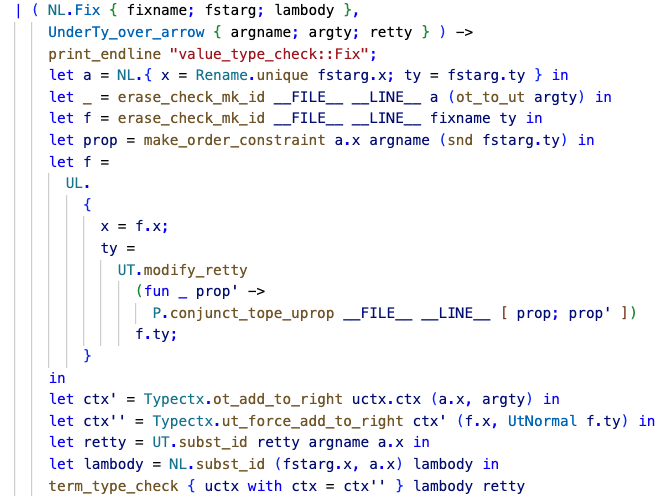
\includegraphics[scale=.35]{fix.png}


\subsection{Supporting Red-Black Trees}
Base Typing
\begin{lstlisting}[language=caml, basicstyle=\small\ttfamily]
type 'a rbtree = Rbleaf
| Rbnode of (color: color;
            val: a';
            ltree : 'a rbtree;
            rtree: 'a rbtree)
\end{lstlisting}

Program underapprox spec
\begin{lstlisting}[language=caml, basicstyle=\small\ttfamily]
external method_predicates :
    t = "numblack" "hdcolor" "noredred"

let rbtree_gen =
  let inv = (v >= 0 : [%v: int]) [@over] in
  let c = (true : [%v: bool]) [@over] in
  let height =
    (v >= 0 &&
      implies c (v + v == inv) &&
      implies (not c) (v + v + 1 == inv)
      : [%v: int]) [@over]
  in
  (* the height is the number of black nodes *)
  (numblack v height &&
    noredred v &&
    fun (u : [%forall: int]) ->
   (* parent is red; the hdcolor cannot be red *)
   (c && not (hdcolor v true)) ||
   (* parent is black; the hdcolor can be any color *)
   ((not c) &&
    implies (height == 0) (hdcolor v true))
    : [%v: int rbtree]) [@under]
\end{lstlisting}

\subsection{Timeouts}


\end{document}
\endinput
